\documentclass[11pt,a4paper,]{article}
\usepackage{lmodern}

\usepackage{amssymb,amsmath}
\usepackage{ifxetex,ifluatex}
\usepackage{fixltx2e} % provides \textsubscript
\ifnum 0\ifxetex 1\fi\ifluatex 1\fi=0 % if pdftex
  \usepackage[T1]{fontenc}
  \usepackage[utf8]{inputenc}
\else % if luatex or xelatex
  \usepackage{unicode-math}
  \defaultfontfeatures{Ligatures=TeX,Scale=MatchLowercase}
\fi
% use upquote if available, for straight quotes in verbatim environments
\IfFileExists{upquote.sty}{\usepackage{upquote}}{}
% use microtype if available
\IfFileExists{microtype.sty}{%
\usepackage[]{microtype}
\UseMicrotypeSet[protrusion]{basicmath} % disable protrusion for tt fonts
}{}
\PassOptionsToPackage{hyphens}{url} % url is loaded by hyperref
\usepackage[unicode=true]{hyperref}
\hypersetup{
            pdftitle={Offences in Australis (2008 - 2018)},
            pdfborder={0 0 0},
            breaklinks=true}
\urlstyle{same}  % don't use monospace font for urls
\usepackage{geometry}
\geometry{a4paper, centering, text={16cm,24cm}}
\usepackage[style=authoryear-comp,]{biblatex}
\addbibresource{references.bib}
\usepackage{longtable,booktabs}
% Fix footnotes in tables (requires footnote package)
\IfFileExists{footnote.sty}{\usepackage{footnote}\makesavenoteenv{long table}}{}
\usepackage{graphicx,grffile}
\makeatletter
\def\maxwidth{\ifdim\Gin@nat@width>\linewidth\linewidth\else\Gin@nat@width\fi}
\def\maxheight{\ifdim\Gin@nat@height>\textheight\textheight\else\Gin@nat@height\fi}
\makeatother
% Scale images if necessary, so that they will not overflow the page
% margins by default, and it is still possible to overwrite the defaults
% using explicit options in \includegraphics[width, height, ...]{}
\setkeys{Gin}{width=\maxwidth,height=\maxheight,keepaspectratio}
\IfFileExists{parskip.sty}{%
\usepackage{parskip}
}{% else
\setlength{\parindent}{0pt}
\setlength{\parskip}{6pt plus 2pt minus 1pt}
}
\setlength{\emergencystretch}{3em}  % prevent overfull lines
\providecommand{\tightlist}{%
  \setlength{\itemsep}{0pt}\setlength{\parskip}{0pt}}
\setcounter{secnumdepth}{5}

% set default figure placement to htbp
\makeatletter
\def\fps@figure{htbp}
\makeatother


\title{Offences in Australis (2008 - 2018)}

%% MONASH STUFF

%% CAPTIONS
\RequirePackage{caption}
\DeclareCaptionStyle{italic}[justification=centering]
 {labelfont={bf},textfont={it},labelsep=colon}
\captionsetup[figure]{style=italic,format=hang,singlelinecheck=true}
\captionsetup[table]{style=italic,format=hang,singlelinecheck=true}


%% FONT
\RequirePackage{bera}
\RequirePackage[charter,expert,sfscaled]{mathdesign}
\RequirePackage{fontawesome}

%% HEADERS AND FOOTERS
\RequirePackage{fancyhdr}
\pagestyle{fancy}
\rfoot{\Large\sffamily\raisebox{-0.1cm}{\textbf{\thepage}}}
\makeatletter
\lhead{\textsf{\expandafter{\@title}}}
\makeatother
\rhead{}
\cfoot{}
\setlength{\headheight}{15pt}
\renewcommand{\headrulewidth}{0.4pt}
\renewcommand{\footrulewidth}{0.4pt}
\fancypagestyle{plain}{%
\fancyhf{} % clear all header and footer fields
\fancyfoot[C]{\sffamily\thepage} % except the center
\renewcommand{\headrulewidth}{0pt}
\renewcommand{\footrulewidth}{0pt}}

%% MATHS
\RequirePackage{bm,amsmath}
\allowdisplaybreaks

%% GRAPHICS
\RequirePackage{graphicx}
\setcounter{topnumber}{2}
\setcounter{bottomnumber}{2}
\setcounter{totalnumber}{4}
\renewcommand{\topfraction}{0.85}
\renewcommand{\bottomfraction}{0.85}
\renewcommand{\textfraction}{0.15}
\renewcommand{\floatpagefraction}{0.8}


%\RequirePackage[section]{placeins}

%% SECTION TITLES


%% SECTION TITLES (NEW: Changing sections and subsections color)
\RequirePackage[compact,sf,bf]{titlesec}
\titleformat*{\section}{\Large\sf\bfseries\color[rgb]{0.8, 0.7, 0.1 }}
\titleformat*{\subsection}{\large\sf\bfseries\color[rgb]{0.8, 0.7, 0.1 }}
\titleformat*{\subsubsection}{\sf\bfseries\color[rgb]{0.8, 0.7, 0.1 }}
\titlespacing{\section}{0pt}{2ex}{.5ex}
\titlespacing{\subsection}{0pt}{1.5ex}{0ex}
\titlespacing{\subsubsection}{0pt}{.5ex}{0ex}


%% TITLE PAGE
\def\Date{\number\day}
\def\Month{\ifcase\month\or
 January\or February\or March\or April\or May\or June\or
 July\or August\or September\or October\or November\or December\fi}
\def\Year{\number\year}

%% LINE AND PAGE BREAKING
\sloppy
\clubpenalty = 10000
\widowpenalty = 10000
\brokenpenalty = 10000
\RequirePackage{microtype}

%% PARAGRAPH BREAKS
\setlength{\parskip}{1.4ex}
\setlength{\parindent}{0em}

%% HYPERLINKS
\RequirePackage{xcolor} % Needed for links
\definecolor{darkblue}{rgb}{0,0,.6}
\RequirePackage{url}

\makeatletter
\@ifpackageloaded{hyperref}{}{\RequirePackage{hyperref}}
\makeatother
\hypersetup{
     citecolor=0 0 0,
     breaklinks=true,
     bookmarksopen=true,
     bookmarksnumbered=true,
     linkcolor=darkblue,
     urlcolor=blue,
     citecolor=darkblue,
     colorlinks=true}

\usepackage[showonlyrefs]{mathtools}
\usepackage[no-weekday]{eukdate}

%% BIBLIOGRAPHY

\makeatletter
\@ifpackageloaded{biblatex}{}{\usepackage[style=authoryear-comp, backend=biber, natbib=true]{biblatex}}
\makeatother
\ExecuteBibliographyOptions{bibencoding=utf8,minnames=1,maxnames=3, maxbibnames=99,dashed=false,terseinits=true,giveninits=true,uniquename=false,uniquelist=false,doi=false, isbn=false,url=true,sortcites=false}

\DeclareFieldFormat{url}{\texttt{\url{#1}}}
\DeclareFieldFormat[article]{pages}{#1}
\DeclareFieldFormat[inproceedings]{pages}{\lowercase{pp.}#1}
\DeclareFieldFormat[incollection]{pages}{\lowercase{pp.}#1}
\DeclareFieldFormat[article]{volume}{\mkbibbold{#1}}
\DeclareFieldFormat[article]{number}{\mkbibparens{#1}}
\DeclareFieldFormat[article]{title}{\MakeCapital{#1}}
\DeclareFieldFormat[article]{url}{}
%\DeclareFieldFormat[book]{url}{}
%\DeclareFieldFormat[inbook]{url}{}
%\DeclareFieldFormat[incollection]{url}{}
%\DeclareFieldFormat[inproceedings]{url}{}
\DeclareFieldFormat[inproceedings]{title}{#1}
\DeclareFieldFormat{shorthandwidth}{#1}
%\DeclareFieldFormat{extrayear}{}
% No dot before number of articles
\usepackage{xpatch}
\xpatchbibmacro{volume+number+eid}{\setunit*{\adddot}}{}{}{}
% Remove In: for an article.
\renewbibmacro{in:}{%
  \ifentrytype{article}{}{%
  \printtext{\bibstring{in}\intitlepunct}}}

\AtEveryBibitem{\clearfield{month}}
\AtEveryCitekey{\clearfield{month}}

\makeatletter
\DeclareDelimFormat[cbx@textcite]{nameyeardelim}{\addspace}
\makeatother

\author{\sf\Large\textbf{ Jiang Yiwen}\\ {\sf\large BA\\[0.5cm]} \sf\Large\textbf{ Reports XXXX}\\ {\sf\large XXX\\[0.5cm]} \sf\Large\textbf{ XXX XXX}\\ {\sf\large XXX\\[0.5cm]}}

\date{\sf\Date~\Month~\Year}
\makeatletter
\lfoot{\sf Yiwen, XXXX, XXX: \@date}
\makeatother


%%%% PAGE STYLE FOR FRONT PAGE OF REPORTS

\makeatletter
\def\organization#1{\gdef\@organization{#1}}
\def\telephone#1{\gdef\@telephone{#1}}
\def\email#1{\gdef\@email{#1}}
\makeatother
  \organization{Australian Bureau of Statistic}

  \def\name{Our consultancy \newline add names \&\newline add names}

  \telephone{(03) 9905 2478}

  \email{questions@company.com}                 %NEW: New email addresss

\def\webaddress{\url{http://company.com/stats/consulting/}} %NEW: URl
\def\abn{12 377 614 630}                                    % NEW: ABN
\def\logo{\includegraphics[width=6cm]{logo}}  %NEW: Changing logo
\def\extraspace{\vspace*{1.6cm}}
\makeatletter
\def\contactdetails{\faicon{phone} & \@telephone \\
                    \faicon{envelope} & \@email}
\makeatother

%%%% FRONT PAGE OF REPORTS

\def\reporttype{Report for}

\long\def\front#1#2#3{
\newpage
\begin{singlespacing}
\thispagestyle{empty}
\vspace*{-1.4cm}
\hspace*{-1.4cm}
\hbox to 16cm{
  \hbox to 6.5cm{\vbox to 14cm{\vbox to 25cm{
    \logo
    \vfill
    \parbox{6.3cm}{\raggedright
      \sf\color[rgb]{0.8, 0.7, 0.1 }    % NEW color 
      {\large\textbf{\name}}\par
      \vspace{.7cm}
      \tabcolsep=0.12cm\sf\small
      \begin{tabular}{@{}ll@{}}\contactdetails
      \end{tabular}
      \vspace*{0.3cm}\par
      ABN: \abn\par
    }
  }\vss}\hss}
  \hspace*{0.2cm}
  \hbox to 1cm{\vbox to 14cm{\rule{4pt}{26.8cm}\vss}\hss\hfill}  %NEW: Thicker line
  \hbox to 10cm{\vbox to 14cm{\vbox to 25cm{   
      \vspace*{3cm}\sf\raggedright
      \parbox{11cm}{\sf\raggedright\baselineskip=1.2cm
         \fontsize{24.88}{30}\color[rgb]{0, 0.29, 0.55}\sf\textbf{#1}}   % NEW: title color blue
      \par
      \vfill
      \large
      \vbox{\parskip=0.8cm #2}\par
      \vspace*{2cm}\par
      \reporttype\\[0.3cm]
      \hbox{#3}%\\[2cm]\
      \vspace*{1cm}
      {\large\sf\textbf{\Date~\Month~\Year}}
   }\vss}
  }}
\end{singlespacing}
\newpage
}

\makeatletter
\def\titlepage{\front{\expandafter{\@title}}{\@author}{\@organization}}
\makeatother

\usepackage{setspace}
\setstretch{1.5}

%% Any special functions or other packages can be loaded here.
\usepackage{float}
\let\origfigure\figure
\let\endorigfigure\endfigure
\renewenvironment{figure}[1][2] {
\expandafter\origfigure\expandafter[H]
} {
\endorigfigure
}
\usepackage{booktabs}
\usepackage{longtable}
\usepackage{array}
\usepackage{multirow}
\usepackage{wrapfig}
\usepackage{float}
\usepackage{colortbl}
\usepackage{pdflscape}
\usepackage{tabu}
\usepackage{threeparttable}
\usepackage{threeparttablex}
\usepackage[normalem]{ulem}
\usepackage{makecell}
\usepackage{xcolor}


\begin{document}
\titlepage

\hypertarget{introduction}{%
\section{Introduction}\label{introduction}}

\hypertarget{analysis}{%
\section{Analysis}\label{analysis}}

\section*{Gender difference in the number and rate of offences}

\begin{figure}
\centering
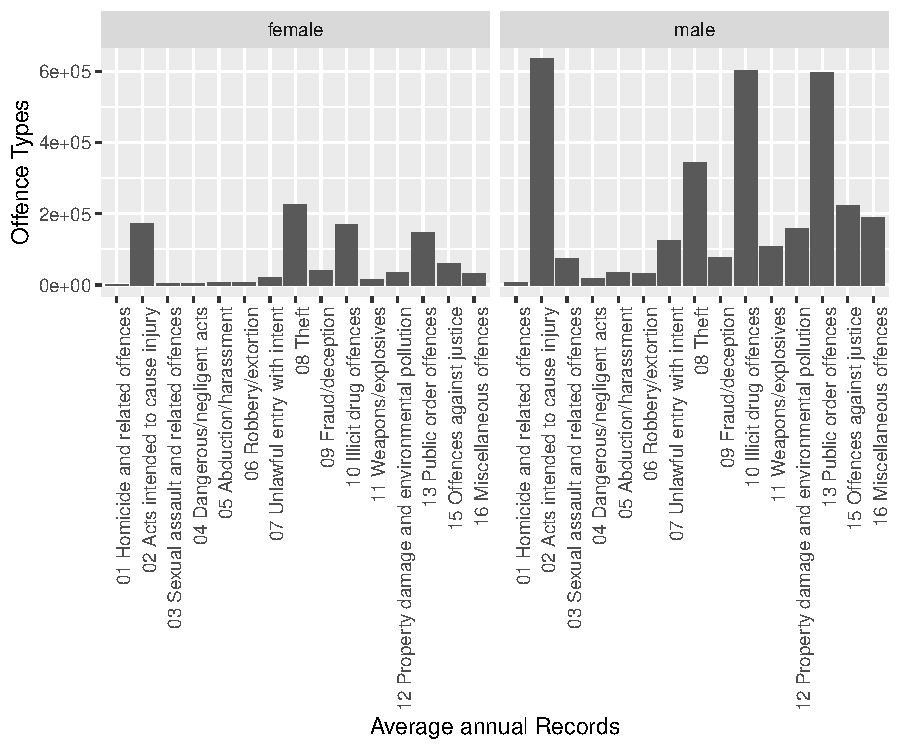
\includegraphics{ETC5513-Assignment4_files/figure-latex/gender1-1.pdf}
\caption{\label{fig:gender1}Yearly average offence records of different offence type}
\end{figure}

As showing in Figure \ref{fig:gender1}, each bar represents the average number of records for each type of offence and gender over the ten years. The overall offence recorded that the number of male offenders is significantly higher than female offenders. The highest number of offence type for males are ``Acts intended to cause injury'' and for females are ``Theft''.

\begin{table}[H]

\caption{\label{tab:gendersumm}Summary of yearly average number of offences}
\centering
\resizebox{\linewidth}{!}{
\begin{tabular}[t]{l|r|r|l}
\hline
Offence Type & Male & Female & Result\\
\hline
01 Homicide and related offences & 614.7 & 114.1 & Males are 5.39 times higher\\
\hline
02 Acts intended to cause injury & 57770.5 & 15729.0 & Males are 3.67 times higher\\
\hline
03 Sexual assault and related offences & 6756.7 & 397.2 & Males are 17.01 times higher\\
\hline
04 Dangerous/negligent acts & 1650.2 & 360.5 & Males are 4.58 times higher\\
\hline
05 Abduction/harassment & 3320.8 & 728.9 & Males are 4.56 times higher\\
\hline
06 Robbery/extortion & 3034.2 & 556.7 & Males are 5.45 times higher\\
\hline
07 Unlawful entry with intent & 11305.4 & 2005.5 & Males are 5.64 times higher\\
\hline
08 Theft & 31245.6 & 20435.6 & Males are 1.53 times higher\\
\hline
09 Fraud/deception & 7029.2 & 3732.1 & Males are 1.88 times higher\\
\hline
10 Illicit drug offences & 54745.5 & 15374.8 & Males are 3.56 times higher\\
\hline
11 Weapons/explosives & 9737.7 & 1443.4 & Males are 6.75 times higher\\
\hline
12 Property damage and environmental pollution & 14539.6 & 3268.2 & Males are 4.45 times higher\\
\hline
13 Public order offences & 54268.5 & 13303.9 & Males are 4.08 times higher\\
\hline
15 Offences against justice & 20230.7 & 5397.5 & Males are 3.75 times higher\\
\hline
16 Miscellaneous offences & 17153.3 & 2975.1 & Males are 5.77 times higher\\
\hline
Total & 308136.3 & 90450.5 & Males are 3.41 times higher\\
\hline
\end{tabular}}
\end{table}

If we look at the summary (Refer to Table \ref{tab:gendersumm}), the result also indicates that in all the offence types, the number of male offenders is significantly higher than female offenders. The ``Sexual assault and related offence'' is the most significant difference between the number of males and females, and the average number of males is about 17 times higher than females. The difference in ``Theft'' is relatively minimal; males are about 1.53 times higher than females. Over the ten years, the average number of male offenders is 4.42 times higher than that of females.

\begin{figure}
\centering
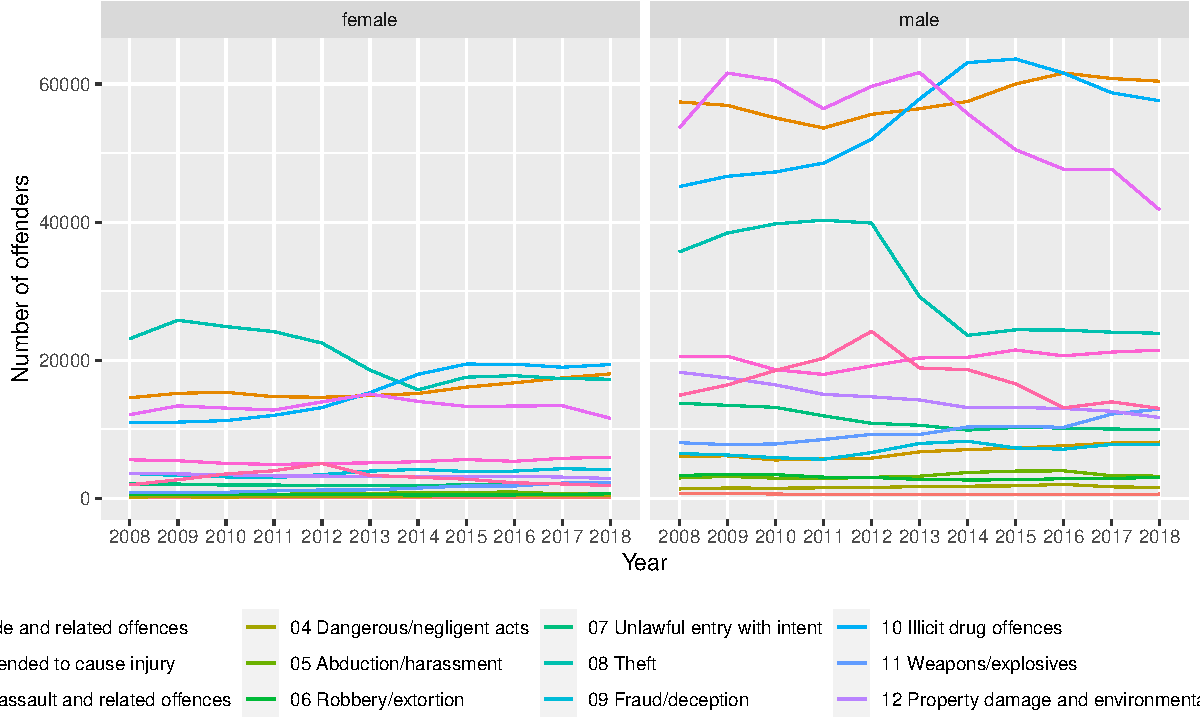
\includegraphics{ETC5513-Assignment4_files/figure-latex/gender2-1.pdf}
\caption{\label{fig:gender2}Yearly Number of Offenders on Female and Male}
\end{figure}

From Figure \ref{fig:gender2}, we can observe that the yearly changes on the number of records of most types of the offence are stable on both genders. However, there still have some changes. For females, the number of ``Theft'' drop highly, from about 25,000 reduced to 15,000 and ``Illicit drug offences'' increased by nearly 10,000. For males, although some type offences remain at a relatively high level, ``Unlawful entry with intent and Property damage'' and ``environmental pollution'' have decreased by about 20,000. Government still need to pay attention to the issue of ``Illicit drug offences'', because the number of records has increased a lot compared to 2008.

\begin{figure}
\centering
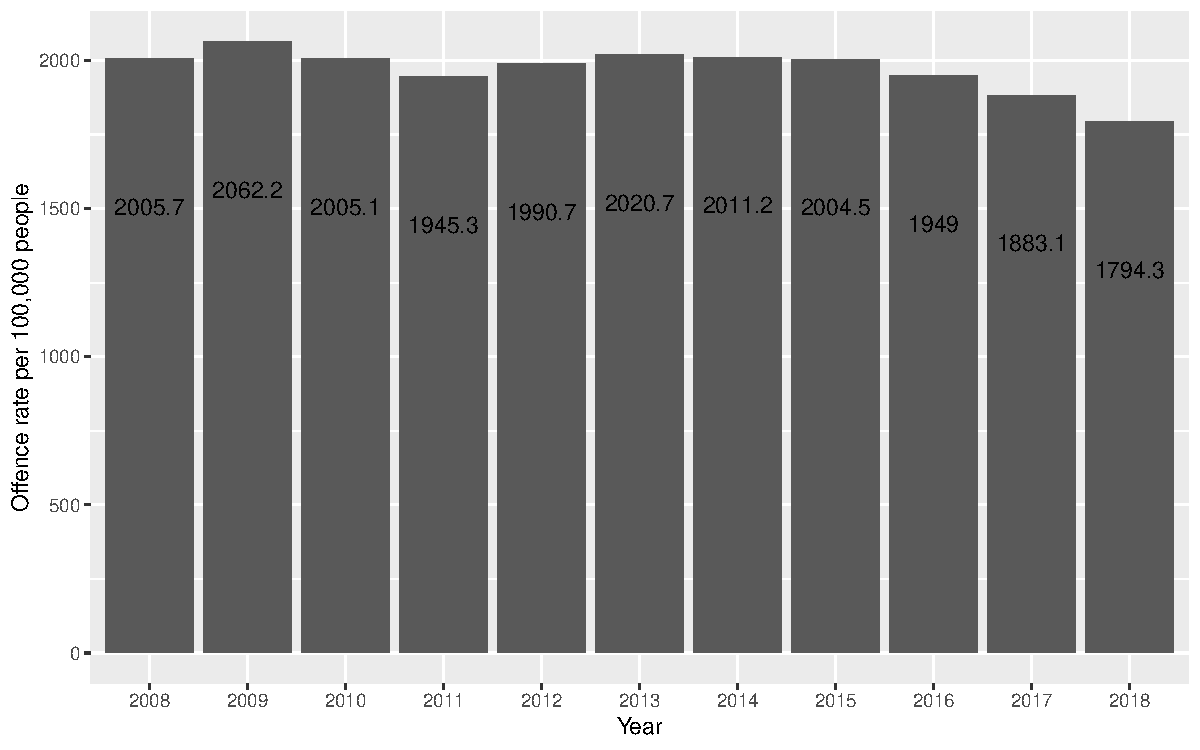
\includegraphics{ETC5513-Assignment4_files/figure-latex/gender3-1.pdf}
\caption{\label{fig:gender3}Rate of offenders recorded in Australia}
\end{figure}

In Figure \ref{fig:gender3}, it represents the offender rate on both genders; the rate indicates the number of offenders in 100,000 people. In 2009, the rate was 2,062 offenders in 100,000 people. After the overall trend is decreasing, in 2018, there are about 1,794 offenders in 100,000 people. The rate decreased to their lowest levels in six years.

\begin{table}[H]

\caption{\label{tab:gendersumm2}Yearly change rate of offence rate}
\centering
\begin{tabu} to \linewidth {>{\raggedright}X>{\raggedleft}X>{\raggedleft}X}
\hline
Year & Rate of male & Rate of female\\
\hline
2018 & -0.0516427 & -0.0354850\\
\hline
2017 & -0.0347731 & -0.0249341\\
\hline
2016 & -0.0354036 & -0.0029570\\
\hline
2015 & -0.0142071 & 0.0372600\\
\hline
2014 & -0.0057571 & 0.0025054\\
\hline
2013 & 0.0159161 & 0.0159667\\
\hline
2012 & 0.0276546 & 0.0072253\\
\hline
2011 & -0.0313991 & -0.0225538\\
\hline
2010 & -0.0274735 & -0.0273654\\
\hline
2009 & 0.0230747 & 0.0428654\\
\hline
\end{tabu}
\end{table}

Focus on the change on the genders (Refer to Table \ref{tab:gendersumm2}); the rate of both genders offenders is continuously decreasing in recent years.

\begin{table}[H]

\caption{\label{tab:gendersumm3}Difference and change rate on number and rate of offence between 2008 to 2018}
\centering
\begin{tabu} to \linewidth {>{\raggedright}X>{\raggedright}X>{\raggedleft}X>{\raggedleft}X}
\toprule
 & Gender & Difference & Growth Rate\\
\midrule
Number of Offender & male & 5239.0 & 0.0178715\\
Number of Offender & female & 13594.0 & 0.1662631\\
Rate of Offender & male & -408.4 & -0.1292691\\
Rate of Offender & female & -9.3 & -0.0107452\\
\bottomrule
\end{tabu}
\end{table}

From Table \ref{tab:gendersumm3}, we can conclude that the number of offenders recorded in Australia increased on both males and females from 2008 to 2018. However, the rate of offenders recorded has dropped significantly, and the offence rate of males has decreased more than that of females.

\begin{itemize}
\tightlist
\item
  The number of male offenders increased by 5,239, and the increasing rate is 1.79\%.\\
\item
  The number of female offenders increased by 13,595, and the increasing rate is 16.63\%.\\
\item
  The rate of male offenders has dropped by 408 per 100,000 people, and the decreasing rate is 12.93\%.\\
\item
  The rate of female offenders has dropped by 9 per 100,000 people, and the decreasing rate is 1.07\%.
\end{itemize}

\section*{body 2}

\section*{body 3}

\hypertarget{conclusion}{%
\section{Conclusion}\label{conclusion}}

\printbibliography[title=Reference]

\end{document}

